\documentclass[8pt,aspectratio=169]{beamer}
\usetheme{Madrid}
\usepackage{graphicx,booktabs,adjustbox,multicol,amsmath,amssymb,listings,xcolor}
\definecolor{mlblue}{RGB}{0,102,204}
\definecolor{mlpurple}{RGB}{51,51,178}
\definecolor{mllavender}{RGB}{173,173,224}
\definecolor{mllavender2}{RGB}{193,193,232}
\definecolor{mllavender3}{RGB}{204,204,235}
\definecolor{mllavender4}{RGB}{214,214,239}
\definecolor{mlorange}{RGB}{255,127,14}
\definecolor{mlgreen}{RGB}{44,160,44}
\definecolor{mlred}{RGB}{214,39,40}
\definecolor{mlgray}{RGB}{127,127,127}
\definecolor{solkeyword}{RGB}{0,102,153}
\setbeamercolor{palette primary}{bg=mllavender3,fg=mlpurple}
\setbeamercolor{palette secondary}{bg=mllavender2,fg=mlpurple}
\setbeamercolor{palette tertiary}{bg=mllavender,fg=white}
\setbeamercolor{palette quaternary}{bg=mlpurple,fg=white}
\setbeamercolor{structure}{fg=mlpurple}
\setbeamercolor{title}{fg=mlpurple}
\setbeamercolor{frametitle}{fg=mlpurple,bg=mllavender3}
\setbeamercolor{block title}{bg=mllavender2,fg=mlpurple}
\setbeamercolor{block body}{bg=mllavender4,fg=black}
\setbeamertemplate{navigation symbols}{}
\setbeamertemplate{itemize items}[circle]
\setbeamersize{text margin left=5mm,text margin right=5mm}
\newcommand{\bottomnote}[1]{\vfill\vspace{-2mm}\textcolor{mllavender2}{\rule{\textwidth}{0.4pt}}\vspace{1mm}\footnotesize\textbf{#1}}
\usepackage{tikz,pgfplots}
\pgfplotsset{compat=1.18}
\usetikzlibrary{arrows.meta,positioning,shapes.geometric,calc}
\title{Ethereum \& Smart Contracts: Course Preview}
\subtitle{INTRO Preview}
\author{Prof.~Dr.~Joerg Osterrieder}
\institute{University Lecture Series}
\date{\today}
\begin{document}

% Frame 1: Title
\begin{frame}
\titlepage
\end{frame}

% Frame 2: Why Ethereum Matters
\begin{frame}{Why Ethereum Matters}
\begin{columns}[T]
\begin{column}{0.62\textwidth}
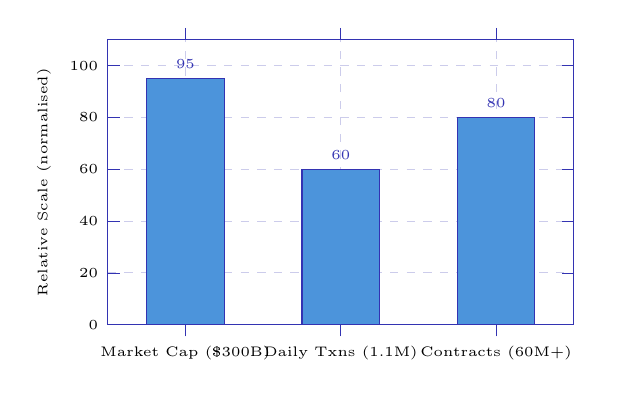
\begin{tikzpicture}
\begin{axis}[
  ybar,
  bar width=28pt,
  width=7.5cm,
  height=5.2cm,
  symbolic x coords={MktCap, DailyTxns, Contracts},
  xtick=data,
  xticklabels={Market Cap (\$300B), Daily Txns (1.1M), Contracts (60M+)},
  xticklabel style={font=\tiny, text width=2.2cm, align=center},
  ymin=0, ymax=110,
  ytick={0,20,40,60,80,100},
  yticklabel style={font=\tiny},
  ylabel style={font=\tiny},
  ylabel={Relative Scale (normalised)},
  axis line style={draw=mlpurple},
  tick style={draw=mlpurple},
  nodes near coords,
  nodes near coords style={font=\tiny, color=mlpurple},
  point meta=y,
  enlarge x limits=0.25,
  grid=major,
  grid style={dashed, mllavender3},
]
\addplot[fill=mlblue!70, draw=mlpurple] coordinates {
  (MktCap,    95)
  (DailyTxns, 60)
  (Contracts, 80)
};
\end{axis}
\end{tikzpicture}
\end{column}
\begin{column}{0.36\textwidth}
\vspace{4mm}
\begin{block}{Key Metrics}
\begin{itemize}\setlength\itemsep{4pt}
  \item[\small$\checkmark$] \small \textbf{\$300B+} market capitalisation
  \item[\small$\checkmark$] \small \textbf{1.1M+} transactions per day
  \item[\small$\checkmark$] \small \textbf{60M+} smart contracts deployed
  \item[\small$\checkmark$] \small \textbf{\$50B+} TVL in DeFi protocols
\end{itemize}
\end{block}
\end{column}
\end{columns}
\vspace{2mm}
\begin{center}
  \textcolor{mlpurple}{\textbf{Ethereum: The backbone of Web3 and decentralised finance}}
\end{center}
\end{frame}

% Frame 3: Course Roadmap
\begin{frame}{Course Roadmap}
\vspace{2mm}
\begin{center}
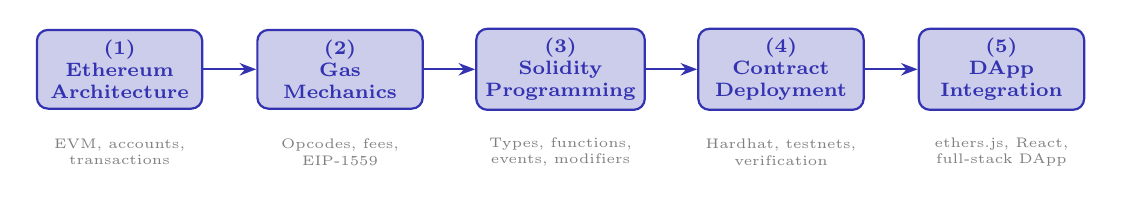
\begin{tikzpicture}[
  procstep/.style={
    rectangle, rounded corners=4pt,
    minimum width=2.1cm, minimum height=1.0cm,
    draw=mlpurple, thick,
    fill=mllavender3,
    font=\scriptsize\bfseries,
    align=center,
    text=mlpurple
  },
  conn/.style={-{Stealth[length=6pt]}, thick, draw=mlpurple}
]
\node[procstep] (s1) at (0,0)    {(1)\\Ethereum\\Architecture};
\node[procstep] (s2) at (2.8,0)  {(2)\\Gas\\Mechanics};
\node[procstep] (s3) at (5.6,0)  {(3)\\Solidity\\Programming};
\node[procstep] (s4) at (8.4,0)  {(4)\\Contract\\Deployment};
\node[procstep] (s5) at (11.2,0) {(5)\\DApp\\Integration};

\draw[conn] (s1) -- (s2);
\draw[conn] (s2) -- (s3);
\draw[conn] (s3) -- (s4);
\draw[conn] (s4) -- (s5);

\node[font=\tiny, text=mlgray, align=center, text width=2.1cm] at (0,-1.05)
  {EVM, accounts,\\transactions};
\node[font=\tiny, text=mlgray, align=center, text width=2.1cm] at (2.8,-1.05)
  {Opcodes, fees,\\EIP-1559};
\node[font=\tiny, text=mlgray, align=center, text width=2.1cm] at (5.6,-1.05)
  {Types, functions,\\events, modifiers};
\node[font=\tiny, text=mlgray, align=center, text width=2.1cm] at (8.4,-1.05)
  {Hardhat, testnets,\\verification};
\node[font=\tiny, text=mlgray, align=center, text width=2.1cm] at (11.2,-1.05)
  {ethers.js, React,\\full-stack DApp};
\end{tikzpicture}
\end{center}
\vspace{4mm}
\begin{columns}[T]
\begin{column}{0.48\textwidth}
\begin{block}{Prerequisites}
\begin{itemize}\setlength\itemsep{2pt}
  \item[\small$\checkmark$] \small Basic programming knowledge
  \item[\small$\checkmark$] \small Familiarity with blockchain concepts
\end{itemize}
\end{block}
\end{column}
\begin{column}{0.48\textwidth}
\begin{block}{Outcomes}
\begin{itemize}\setlength\itemsep{2pt}
  \item[\small$\checkmark$] \small Write and deploy smart contracts
  \item[\small$\checkmark$] \small Build end-to-end decentralised apps
\end{itemize}
\end{block}
\end{column}
\end{columns}
\end{frame}

% Frame 4: EVM Architecture Overview
\begin{frame}{EVM Architecture Overview}
\begin{columns}[T]
\begin{column}{0.55\textwidth}
\vspace{2mm}
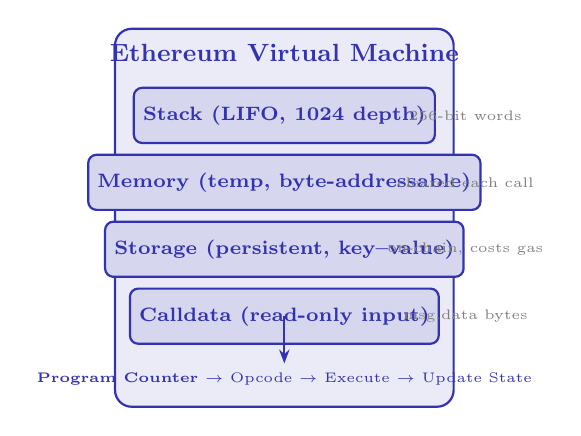
\begin{tikzpicture}[
  mem/.style={rectangle, rounded corners=3pt, draw=mlpurple, thick,
              fill=mllavender4, minimum width=3.6cm, minimum height=0.7cm,
              font=\scriptsize\bfseries, align=center, text=mlpurple},
  lbl/.style={font=\tiny, text=mlgray, align=left},
  conn2/.style={-{Stealth[length=5pt]}, thick, draw=mlpurple}
]
% EVM box
\draw[rounded corners=6pt, draw=mlpurple, thick, fill=mllavender3!40]
  (-0.3,-0.2) rectangle (4.0,4.6);
\node[font=\small\bfseries, text=mlpurple] at (1.85,4.3) {Ethereum Virtual Machine};

\node[mem] (stack)   at (1.85,3.5) {Stack (LIFO, 1024 depth)};
\node[mem] (mem2)    at (1.85,2.65) {Memory (temp, byte-addressable)};
\node[mem] (storage) at (1.85,1.80) {Storage (persistent, key--value)};
\node[mem] (calldata) at (1.85,0.95) {Calldata (read-only input)};

\node[lbl] at (4.15,3.5)  {256-bit words};
\node[lbl] at (4.15,2.65) {cleared each call};
\node[lbl] at (4.15,1.80) {on-chain, costs gas};
\node[lbl] at (4.15,0.95) {msg.data bytes};

\draw[conn2] (1.85,0.95) -- (1.85,0.35);
\node[font=\tiny, text=mlpurple, align=center] at (1.85,0.15)
  {\textbf{Program Counter} $\rightarrow$ Opcode $\rightarrow$ Execute $\rightarrow$ Update State};
\end{tikzpicture}
\end{column}
\begin{column}{0.42\textwidth}
\vspace{2mm}
\begin{block}{Opcode Execution Cycle}
\begin{enumerate}\setlength\itemsep{3pt}
  \item \small \textbf{Fetch}: PC reads next opcode byte
  \item \small \textbf{Decode}: Map opcode to operation
  \item \small \textbf{Execute}: Manipulate stack/memory
  \item \small \textbf{Charge}: Deduct gas cost
  \item \small \textbf{Advance}: Increment PC
\end{enumerate}
\end{block}
\vspace{3mm}
\begin{block}{Two Account Types}
\begin{itemize}\setlength\itemsep{2pt}
  \item[\small$\checkmark$] \small \textbf{EOA}: Externally Owned (private key)
  \item[\small$\checkmark$] \small \textbf{Contract}: Code + Storage, no key
\end{itemize}
\end{block}
\end{column}
\end{columns}
\end{frame}

% Frame 5: Gas Economics at a Glance
\begin{frame}{Gas Economics at a Glance}
\begin{columns}[T]
\begin{column}{0.55\textwidth}
\vspace{1mm}
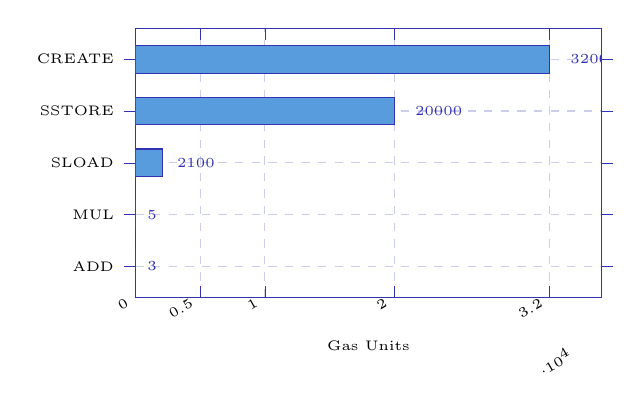
\begin{tikzpicture}
\begin{axis}[
  xbar,
  bar width=10pt,
  width=7.5cm,
  height=5.0cm,
  symbolic y coords={ADD,MUL,SLOAD,SSTORE,CREATE},
  ytick=data,
  yticklabel style={font=\tiny, align=right},
  xmin=0, xmax=36000,
  xtick={0,5000,10000,20000,32000},
  xticklabel style={font=\tiny, rotate=30, anchor=east},
  xlabel style={font=\tiny},
  xlabel={Gas Units},
  axis line style={draw=mlpurple},
  tick style={draw=mlpurple},
  grid=major,
  grid style={dashed, mllavender3},
  enlarge y limits=0.15,
]
\addplot[fill=mlblue!65, draw=mlpurple] coordinates {
  (3,ADD)
  (5,MUL)
  (2100,SLOAD)
  (20000,SSTORE)
  (32000,CREATE)
};
\node[font=\tiny, color=mlpurple, xshift=6pt]  at (axis cs:3,ADD)     {3};
\node[font=\tiny, color=mlpurple, xshift=6pt]  at (axis cs:5,MUL)     {5};
\node[font=\tiny, color=mlpurple, xshift=12pt] at (axis cs:2100,SLOAD)  {2100};
\node[font=\tiny, color=mlpurple, xshift=16pt] at (axis cs:20000,SSTORE) {20000};
\node[font=\tiny, color=mlpurple, xshift=16pt] at (axis cs:32000,CREATE) {32000};
\end{axis}
\end{tikzpicture}
\end{column}
\begin{column}{0.42\textwidth}
\vspace{2mm}
\begin{block}{EIP-1559 Fee Structure}
\begin{center}
\small
\begin{tabular}{@{}ll@{}}
\toprule
\textbf{Component} & \textbf{Destination} \\
\midrule
\texttt{base\_fee} & Burned ($\checkmark$ deflationary) \\
\texttt{priority\_fee} & Validator tip \\
\midrule
\textbf{Total fee} & \texttt{base + priority} \\
\bottomrule
\end{tabular}
\end{center}
\end{block}
\vspace{3mm}
\begin{block}{Gas Formula}
\[
  \text{Cost} = \text{gas\_used} \times (\text{base\_fee} + \text{priority\_fee})
\]
\end{block}
\vspace{2mm}
{\tiny\textcolor{mlgray}{$\star$ Storage ops dominate gas costs --- minimise SSTORE calls}}
\end{column}
\end{columns}
\end{frame}

% Frame 6: What You'll Build
\begin{frame}{What You'll Build}
\vspace{2mm}
\begin{center}
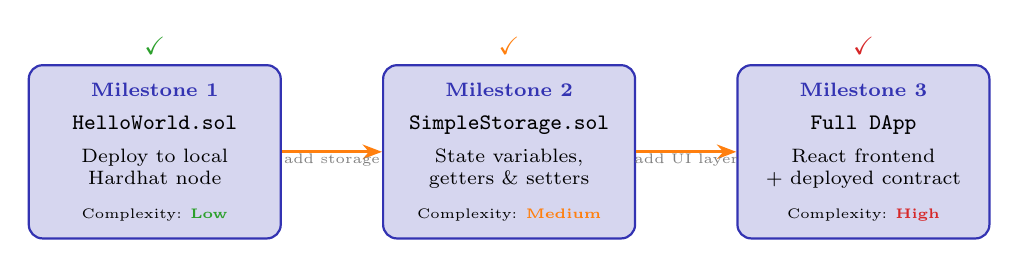
\begin{tikzpicture}[
  card/.style={
    rectangle, rounded corners=5pt,
    draw=mlpurple, thick,
    fill=mllavender4,
    minimum width=3.2cm, minimum height=2.2cm,
    align=center, font=\scriptsize, text=black
  },
  conn3/.style={-{Stealth[length=7pt]}, very thick, draw=mlorange}
]
% Card 1
\node[card] (c1) at (0,0) {
  \textcolor{mlpurple}{\textbf{Milestone 1}}\\[4pt]
  \texttt{\footnotesize HelloWorld.sol}\\[4pt]
  \scriptsize Deploy to local\\
  \scriptsize Hardhat node\\[4pt]
  \tiny Complexity: \textcolor{mlgreen}{\textbf{Low}}
};

% Card 2
\node[card] (c2) at (4.5,0) {
  \textcolor{mlpurple}{\textbf{Milestone 2}}\\[4pt]
  \texttt{\footnotesize SimpleStorage.sol}\\[4pt]
  \scriptsize State variables,\\
  \scriptsize getters \& setters\\[4pt]
  \tiny Complexity: \textcolor{mlorange}{\textbf{Medium}}
};

% Card 3
\node[card] (c3) at (9.0,0) {
  \textcolor{mlpurple}{\textbf{Milestone 3}}\\[4pt]
  \texttt{\footnotesize Full DApp}\\[4pt]
  \scriptsize React frontend\\
  \scriptsize + deployed contract\\[4pt]
  \tiny Complexity: \textcolor{mlred}{\textbf{High}}
};

\draw[conn3] (c1.east) -- (c2.west);
\draw[conn3] (c2.east) -- (c3.west);

% Labels below arrows
\node[font=\tiny, text=mlgray] at (2.25,-0.1) {add storage};
\node[font=\tiny, text=mlgray] at (6.75,-0.1) {add UI layer};

% Checkmarks above
\node[font=\small, text=mlgreen] at (0, 1.35)   {$\checkmark$};
\node[font=\small, text=mlorange] at (4.5, 1.35) {$\checkmark$};
\node[font=\small, text=mlred] at (9.0, 1.35)   {$\checkmark$};
\end{tikzpicture}
\end{center}
\vspace{3mm}
\begin{center}
  \colorbox{mllavender3}{\parbox{0.82\textwidth}{\centering\small
    \textcolor{mlpurple}{\textbf{By the end:}} deploy your own contract on a public testnet
    and interact with it via a live web interface.
  }}
\end{center}
\bottomnote{You already know more than you think --- every expert started with \texttt{HelloWorld}. Let's build!}
\end{frame}

\end{document}
